\documentclass[xcolor=dvipsnames]{beamer}
  \usepackage{eso-pic}
  \usepackage{lmodern}% http://ctan.org/pkg/lm
  \usepackage{fix-cm} % Fixes warnings about missing fonts; see http://tex.stackexchange.com/questions/32378/xfrac-siunitx-gives-me-a-font-warning
  \usepackage{stmaryrd}
  \usepackage{soul}
  \usepackage{amssymb,amsthm,amsmath,amsxtra}
  \usepackage[all]{xy}
  \usepackage{xfrac}
  \usepackage{calc}
  \usepackage{tikz}
  \usetikzlibrary{arrows,calc,automata,shadows,backgrounds,positioning,intersections,fadings,decorations.pathreplacing,shapes,snakes, matrix}
  \usepackage{tikz-cd}
  \tikzset{commutative diagrams/.cd, arrow style = tikz, diagrams = {>=latex}}
  \tikzset{>=latex}
  \usepackage{marvosym}
  \usepackage[marvosym]{tikzsymbols}
  \usepackage{beamerthemesplit}
  \usecolortheme[named=SeaGreen]{structure}
  % \usetheme{Singapore}
  % \setbeamersize{text margin top=-1in}
  \setbeamertemplate{navigation symbols}{}%remove navigation symbols
  \addtolength{\parskip}{0.5\baselineskip}
  \setlength{\arraycolsep}{2pt}
  \DeclareMathOperator{\AJ}{AJ}
  \DeclareMathOperator{\area}{area}
  \DeclareMathOperator{\opchar}{char}
  \DeclareMathOperator{\opdiv}{div}
  \DeclareMathOperator{\grad}{grad}
  \DeclareMathOperator{\Cl}{Cl}
  \DeclareMathOperator{\disc}{disc}
  \DeclareMathOperator{\Gal}{Gal}
  \DeclareMathOperator{\id}{id}
  \DeclareMathOperator{\M}{M}
  \DeclareMathOperator{\tr}{tr}
  \DeclareMathOperator{\nrd}{nrd}
  \DeclareMathOperator{\opP}{P}
  \DeclareMathOperator{\OO}{O}
  \DeclareMathOperator{\PGL}{PGL}
  \DeclareMathOperator{\GL}{GL}
  \DeclareMathOperator{\PSL}{PSL}
  \DeclareMathOperator{\PSU}{PSU}
  \DeclareMathOperator{\SL}{SL}
  \DeclareMathOperator{\SO}{SO}
  \DeclareMathOperator{\vol}{vol}
  \DeclareMathOperator{\Mon}{Mon}
  \DeclareMathOperator{\rad}{rad}
  \newcommand{\quat}[2]{\displaystyle{\bigly(\frac{#1}{#2}\biggr)}}
  \theoremstyle{plain}
  \newtheorem*{thm}{Theorem}
  \newtheorem*{lem}{Lemma}
  \newtheorem*{prop}{Proposition}
  \newtheorem*{ques}{Question}
  \newcommand{\psmod}[1]{~(\textup{\text{mod}}~{#1})}
  \newcommand{\CC}{\mathbb C}
  \newcommand{\A}{\mathbb A}
  \newcommand{\F}{\mathbb F}
  \newcommand{\HH}{\mathbb H}
  \newcommand{\PP}{\mathbb P}
  \newcommand{\R}{\mathbb R}
  \newcommand{\Q}{\mathbb Q}
  \newcommand{\Z}{\mathbb{Z}}
  \newcommand{\Qbar}{\overline{\mathbb Q}}
  \newcommand{\calD}{\mathcal{D}}
  \newcommand{\calG}{\mathcal{G}}
  \newcommand{\calH}{\mathcal H}
  \newcommand{\calO}{\mathcal O}
  \newcommand{\wt}[1]{\widetilde{#1}}
  \newcommand{\defi}[1]{\textbf{#1}} 				% for defined terms
  \setlength{\hfuzz}{4pt}
  \newcommand{\Belyi}{Bely\u{\i}}
  \newcommand{\legen}[2]{\left(\frac{#1}{#2}\right)}

\title{$2$-Solvable \Belyi Maps}
\author{Michael Musty}
\date{}

\newcommand\AtPagemyUpperLeft[1]{\AtPageLowerLeft{%
\put(\LenToUnit{0.87\paperwidth},\LenToUnit{0.815\paperheight}){#1}}}
\newcommand\AtPagemyLowerRight[1]{\AtPageLowerLeft{%
  \put(\LenToUnit{0.88\paperwidth},\LenToUnit{0.02\paperheight}){#1}}}
\AddToShipoutPictureFG{
  \AtPagemyUpperLeft{{
\includegraphics[scale=.081]{chseal-white.png}}}
  \AtPagemyLowerRight{
    \usebeamerfont{framenumber}\insertframenumber{} / \inserttotalframenumber\hspace*{2ex}
  }
}%

\begin{document}
  \begin{frame}[plain]
    \begin{center}{
      \Huge\color{SeaGreen}
      $2$-solvable
      \Belyi\ maps
    }
    \end{center}
    \begin{center}
      %\includegraphics[scale = .3]{4A.pdf}
      %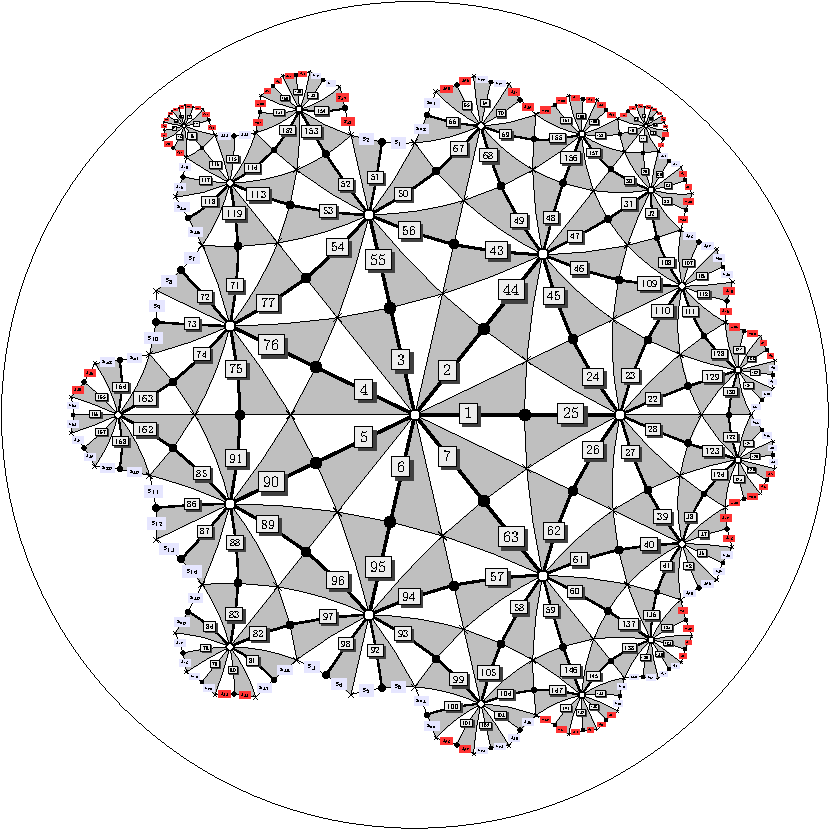
\includegraphics[scale = .3]{168A.pdf}
      %\includegraphics[scale = 0.3]{168Abw.pdf}
      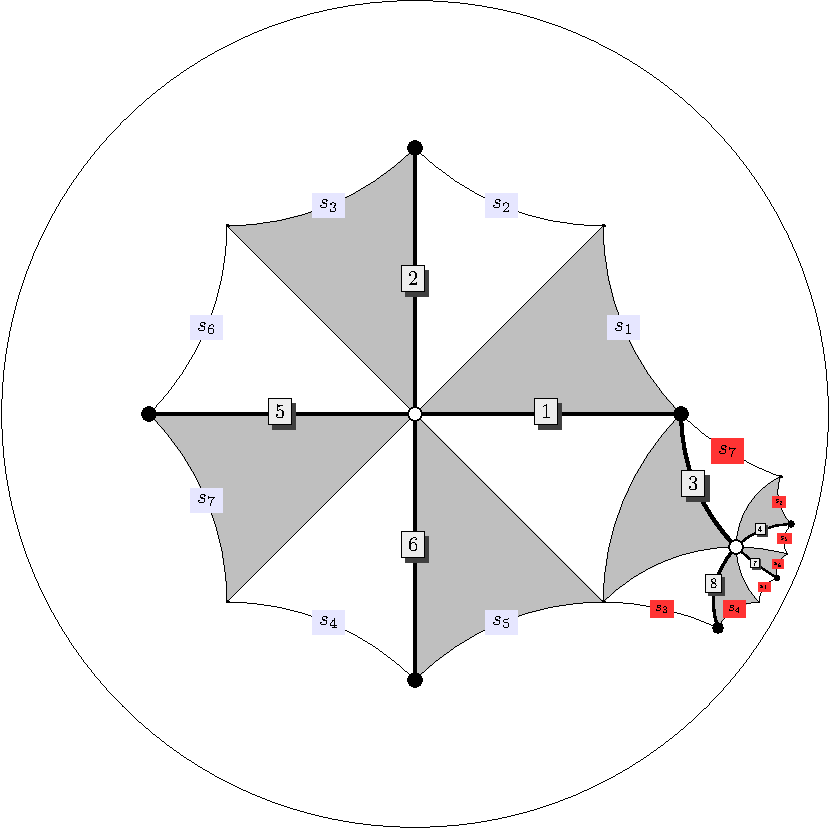
\includegraphics[scale = 0.3]{8T5-g2.pdf}
    \end{center}
    \begin{center}
      Michael Musty\\
      Algebra and Number Theory Seminar\\
      Dartmouth College\\
      May 8, 2018
    \end{center}
  \end{frame}
  \begin{frame}[plain]
    \begin{center}{
      \Huge\color{SeaGreen}
      $2$-solvable
      \Belyi\ maps
    }
    \end{center}
    \begin{center}
      %\includegraphics[scale = .3]{4A.pdf}
      %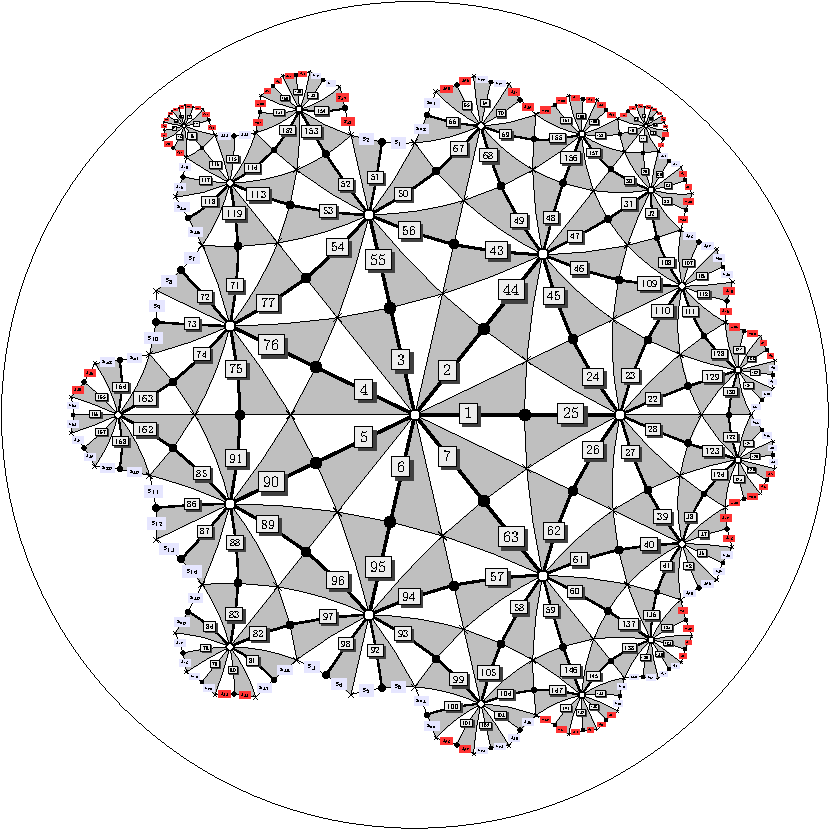
\includegraphics[scale = .3]{168A.pdf}
      %\includegraphics[scale = 0.3]{168Abw.pdf}
      %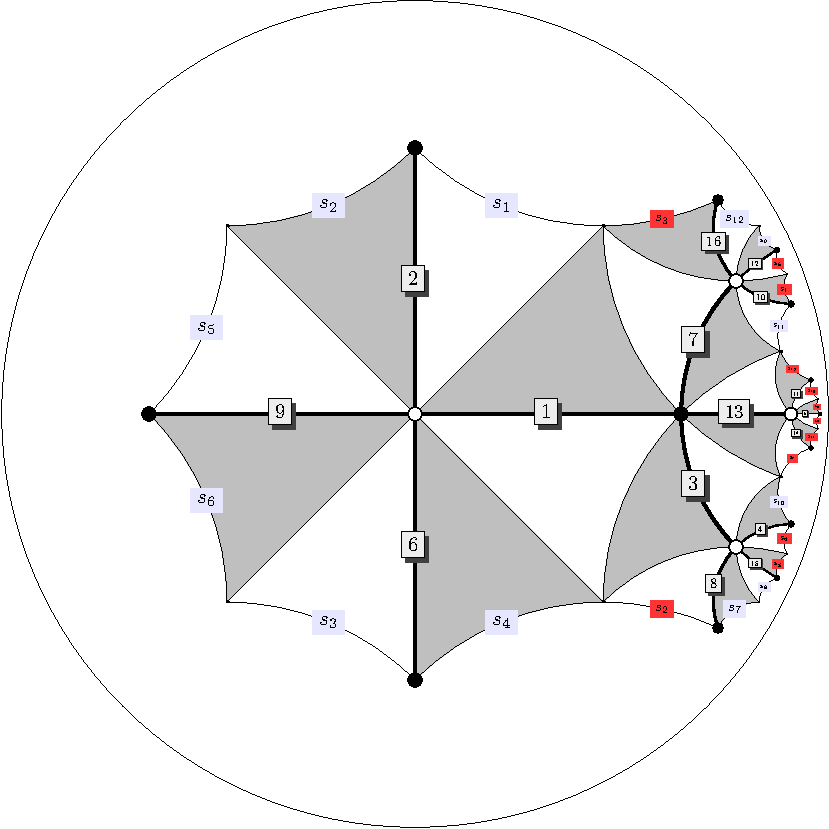
\includegraphics[scale = 0.3]{16T8-g3.pdf}
      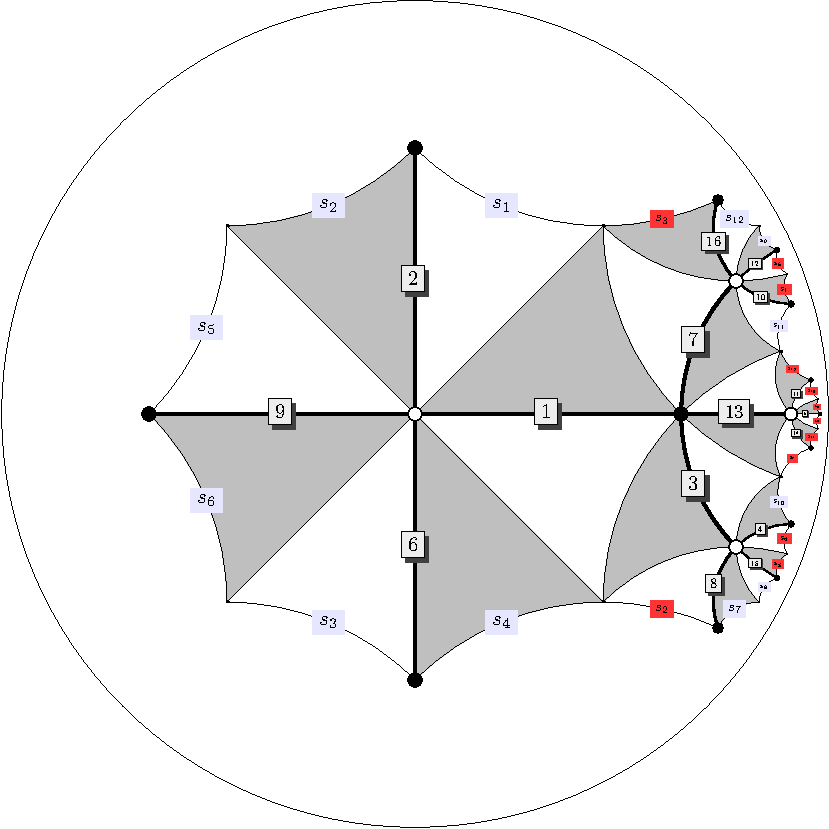
\includegraphics[scale = 0.3]{16T8-g3.pdf}
    \end{center}
    \begin{center}
      Michael Musty\\
      Algebra and Number Theory Seminar\\
      Dartmouth College\\
      May 8, 2018
    \end{center}
  \end{frame}
  \begin{frame}[plain]
    \begin{center}{
      \Huge\color{SeaGreen}
      $2$-solvable
      \Belyi\ maps
    }
    \end{center}
    \begin{center}
      %\includegraphics[scale = .3]{4A.pdf}
      %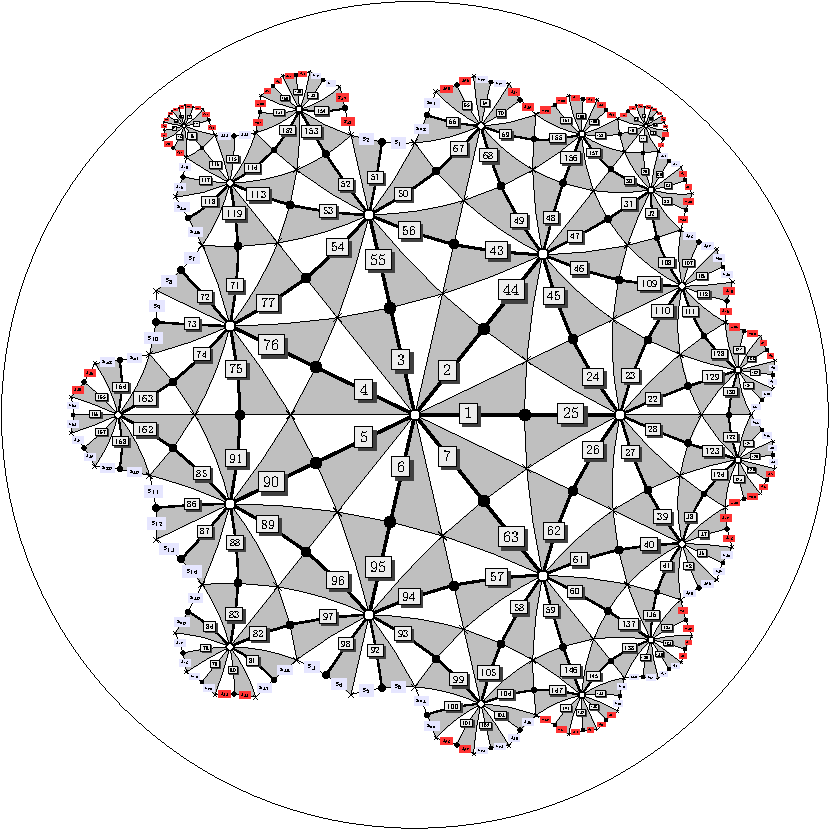
\includegraphics[scale = .3]{168A.pdf}
      %\includegraphics[scale = 0.3]{168Abw.pdf}
      %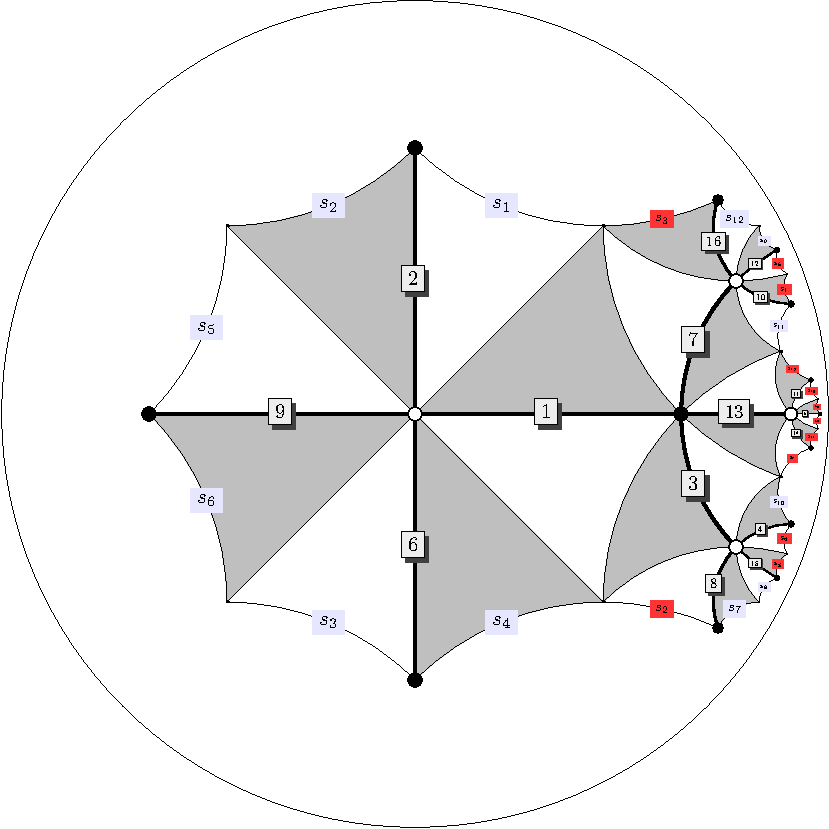
\includegraphics[scale = 0.3]{16T8-g3.pdf}
      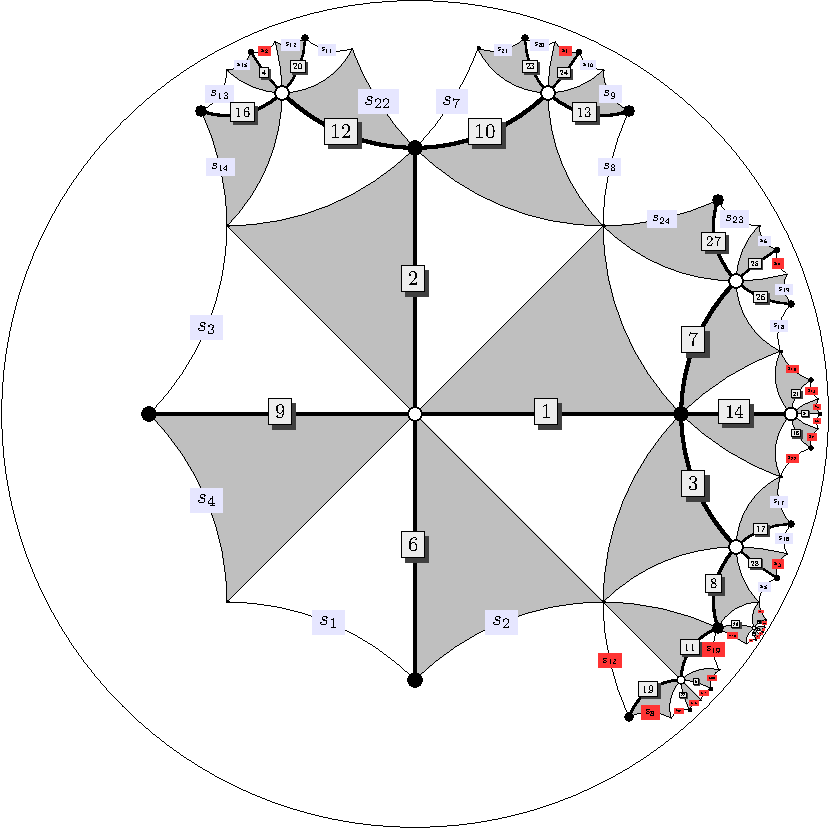
\includegraphics[scale = 0.3]{32S2-g5.pdf}
    \end{center}
    \begin{center}
      Michael Musty\\
      Algebra and Number Theory Seminar\\
      Dartmouth College\\
      May 8, 2018
    \end{center}
  \end{frame}
  \begin{frame}[plain]
    \begin{center}{
      \Huge\color{SeaGreen}
      $2$-solvable
      \Belyi\ maps
    }
    \end{center}
    \begin{center}
      %\includegraphics[scale = .3]{4A.pdf}
      %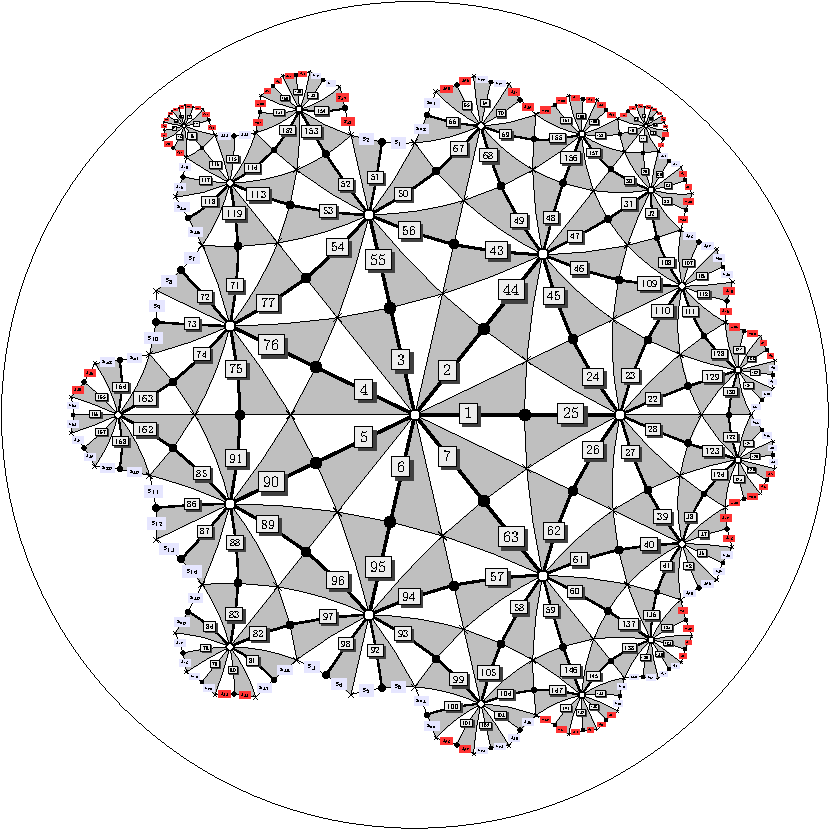
\includegraphics[scale = .3]{168A.pdf}
      %\includegraphics[scale = 0.3]{168Abw.pdf}
      %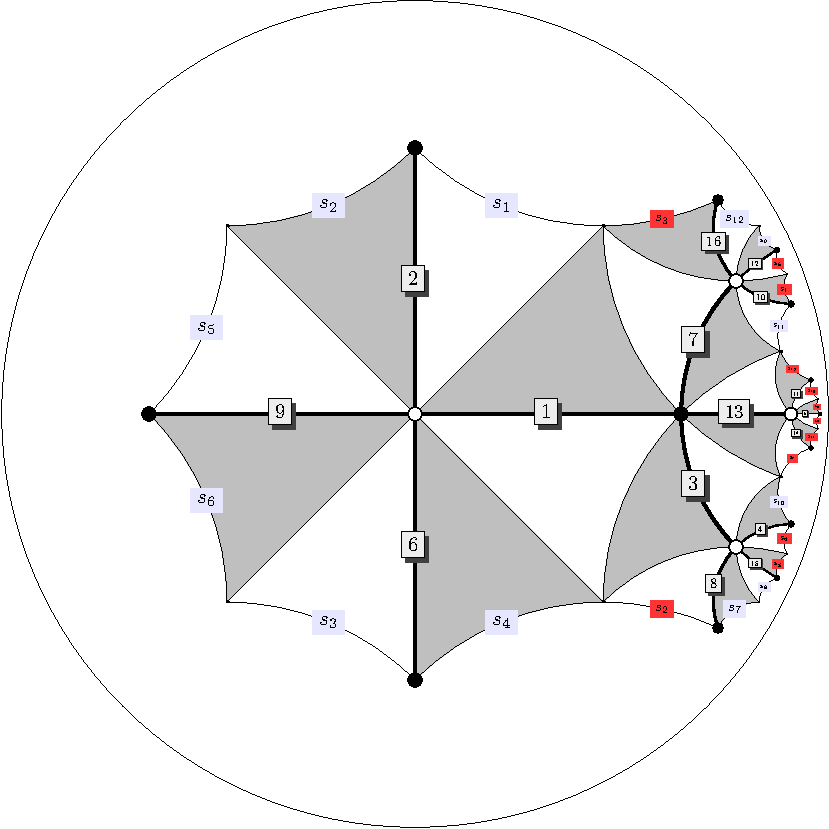
\includegraphics[scale = 0.3]{16T8-g3.pdf}
      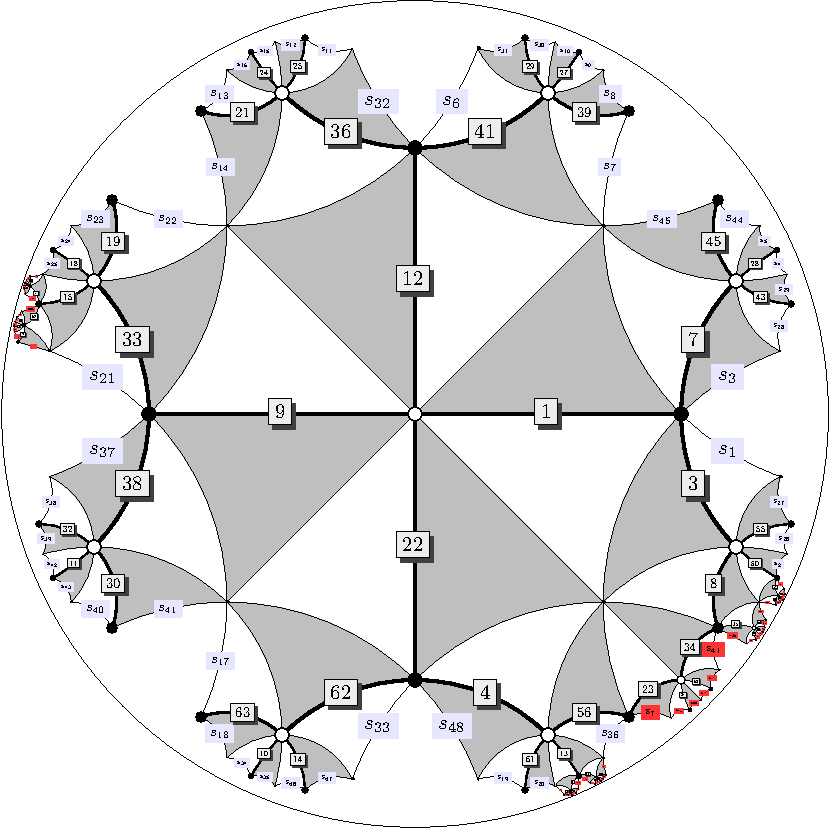
\includegraphics[scale = 0.3]{64S23-g9.pdf}
    \end{center}
    \begin{center}
      Michael Musty\\
      Algebra and Number Theory Seminar\\
      Dartmouth College\\
      May 8, 2018
    \end{center}
  \end{frame}
  \begin{frame}[plain]
    \begin{center}{
      \Huge\color{SeaGreen}
      $2$-solvable
      \Belyi\ maps
    }
    \end{center}
    \begin{center}
      %\includegraphics[scale = .3]{4A.pdf}
      %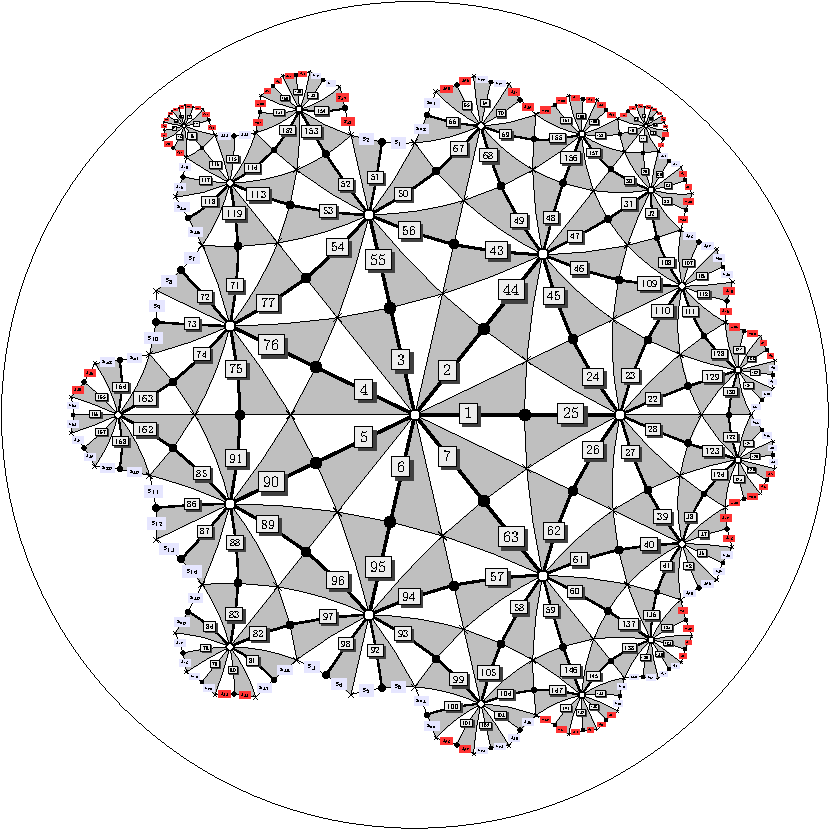
\includegraphics[scale = .3]{168A.pdf}
      %\includegraphics[scale = 0.3]{168Abw.pdf}
      %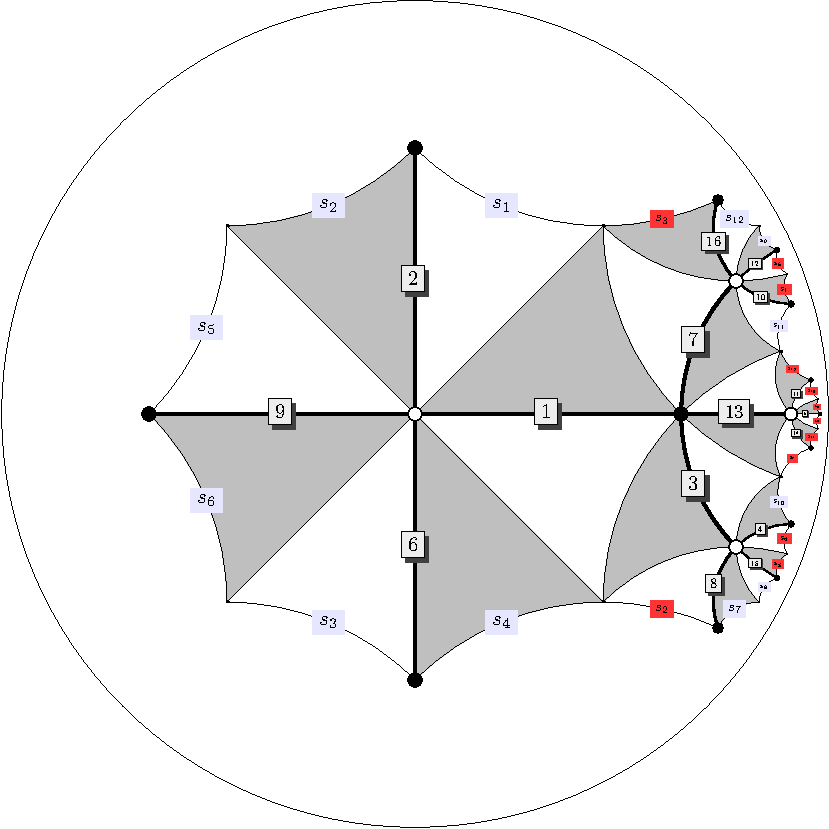
\includegraphics[scale = 0.3]{16T8-g3.pdf}
      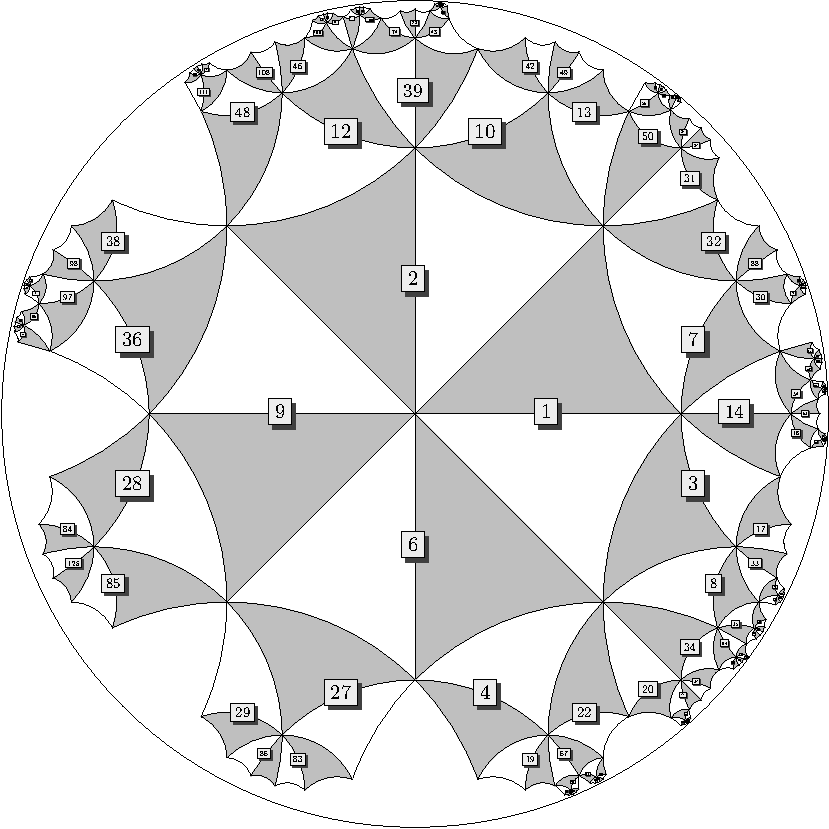
\includegraphics[scale = 0.3]{128S36-g17.pdf}
    \end{center}
    \begin{center}
      Michael Musty\\
      Algebra and Number Theory Seminar\\
      Dartmouth College\\
      May 8, 2018
    \end{center}
  \end{frame}
  \begin{frame}[plain]
    \frametitle{Outline}
    \begin{enumerate}
      \item
        What is a 2-solvable \Belyi\ map?
      \item
        Motivation: Beckmann's Theorem
      \item
        An algorithm to compute 2-solvable \Belyi\ maps
        \begin{enumerate}[(a)]
          \item
            Computing permutation triples
          \item
            Computing equations
        \end{enumerate}
      \item
        Examples
      \item
        Application: Number fields obtained from $2$-torsion points
    \end{enumerate}
  \end{frame}
  \begin{frame}[plain]
    \frametitle{\Belyi's Theorem}
    \pause
    \begin{thm}[G.V. \Belyi\ 1979]
      A smooth projective curve $X$ over $\CC$
      can be defined over $\overline{\Q}$ if and only if there
      exists a branched covering of compact connected Riemann surfaces $\phi:X\to\PP^1$
      unramified (unbranched) above $\PP^1\setminus\{0,1,\infty\}$.
    \end{thm}
    \pause
    Such a map is called a \textbf{\Belyi\ map}.
    \pause
    \par
    Two \Belyi\ maps $\phi:X\to\PP^1$ and $\phi':X'\to\PP^1$ are
    \defi{isomorphic} if there is an isomorphism $\iota:X\to X'$
    such that $\phi'\iota = \phi$.
  \end{frame}
  \begin{frame}[plain]
    \frametitle{Passports of \Belyi\ maps}
    \pause
    A \textbf{passport} $\mathcal{P}$ consists of the data
    $(g,G,\lambda)$ where $g\geq 0$ is an integer,
    $G\leq S_d$ is a transitive subgroup,
    and $\lambda = (\lambda_0,\lambda_1,\lambda_\infty)$
    is a triple of partitions of $d$.
    \pause
    \par
    The passport of a \Belyi\ map $\phi:X\to\PP^1$
    is $(g(X), \Mon(\phi), (\lambda_0,\lambda_1,\lambda_\infty))$
    with $g(X)$ the genus of $X$,
    $\Mon(\phi)$ the monodromy group of $\phi$,
    and the partitions specified by ramification.
    \pause
    \par
    There is an action of $\Gal(\Qbar/\Q)$ on \Belyi\ maps.
    \pause
    This action preserves passports.
  \end{frame}
  \begin{frame}[plain]
    \frametitle{Passports of permutation triples}
    \pause
    A \textbf{transitive permutation triple} is a triple
    \newline
    $\sigma = (\sigma_0,\sigma_1,\sigma_\infty)\in S_d^3$
    with $\langle\sigma\rangle$ a transitive subgroup of $S_d$
    and $\sigma_\infty\sigma_1\sigma_0 = 1$.
    \pause
    \par
    Two such triples $\sigma$ and $\sigma'$ are
    \textbf{simultaneously conjugate} if there exists
    $\tau\in S_d$ with
    $$
    (\tau^{-1}\sigma_0\tau,\tau^{-1}\sigma_1\tau,\tau^{-1}\sigma_\infty\tau) =
    (\sigma_0',\sigma_1',\sigma_\infty').
    $$
    \pause
    The passport of a permutation triple $\sigma$ is
    $(g(\sigma), \langle\sigma\rangle, \lambda(\sigma))$
    \pause
    where
    $$
    g(\sigma) = 1-d+(e(\sigma_0)-e(\sigma_1)-e(\sigma_\infty))/2
    $$
    \pause
    with
    $$
    e(\tau) = d-\#\text{cycles of }\tau,
    $$
    \pause
    and $\lambda(\sigma)$ is specified by cycle structures.
    \pause
    \par
    The \defi{size} of a passport $\mathcal{P}$ is the number of
    simultaneous conjugacy classes of transitive permutation triples
    with passport $\mathcal{P}$.
  \end{frame}
  \begin{frame}[plain]
    \frametitle{A group-theoretic description of \Belyi\ maps}
    \pause
    \begin{lem}
      The set of transitive permutation triples of degree $d$
      up to simultaneous conjugation is in bijection with the
      set of \Belyi\ maps of degree $d$ up to isomorphism.
    \end{lem}
  \end{frame}
  \begin{frame}[plain]
    \frametitle{A Zoo of Bijections}
    \pause
    \begin{center}
      \begin{tikzpicture}[scale=.7]
        \node at (0,0) (dessins)
        {
          $
            \left\{
              \begin{minipage}{11ex}
                dessins with $d$ edges
              \end{minipage}
            \right\}
          $
        };
        \node at (-5,3) (perms)
        {
          $
            \left\{
              \begin{minipage}{22ex}
                Transitive permutation Triples
                $(\sigma_0,\sigma_1,\sigma_\infty)\in S_d^3$
                with $\sigma_\infty\sigma_1\sigma_0 = 1$
              \end{minipage}
            \right\}
          $
        };
        \node at (5,3) (triangles)
        {
          $
            \left\{
              \begin{minipage}{22ex}
                Index $d$ triangle subgroups
                $\Gamma \leq \Delta(a,b,c)$
              \end{minipage}
            \right\}
          $
        };
        \node at (5,-3) (belyis)
        {
          $
            \left\{
              \begin{minipage}{22ex}
                \Belyi\ maps of degree $d$
              \end{minipage}
            \right\}
          $
        };
        \node at (-5,-3) (fields)
        {
          $
            \left\{
              \begin{minipage}{22ex}
                Degree $d$ function
                field extensions $K \supseteq \CC(z)$
                with discriminant supported above $0,1,\infty$
              \end{minipage}
            \right\}
          $
        };
        \draw[<->] (dessins) to node [above,rotate=-35] {$\sim$} node {} (perms);
        \draw[<->] (dessins) to node [above,rotate=-35] {$\sim$} node {} (belyis);
        \draw[<->] (dessins) to node [above,rotate=35] {$\sim$} node {} (triangles);
        \draw[<->] (dessins) to node [above,rotate=35] {$\sim$} node {} (fields);
      \end{tikzpicture}
    \end{center}
    \pause
    All up to the appropriate version of
    equivalence in each category.
  \end{frame}
  \begin{frame}[plain]
    \frametitle{Example \texttt{2T1-2,1,2-g0}}
    \begin{center}
      \begin{tikzpicture}[scale=.37]
        % dashed
          %\draw[blue,ultra thin,dashed] (4,10.5)--(6,15);
        \draw[gray,ultra thin,dashed] (10,13.5)--(12,18);
        \draw[<-,black,thin,dashed] (4,3)--(4,17);
        \draw[<-,black,thin,dashed] (10,3)--(10,13.5);
        % ComplexPlane
        \draw[thick] (0,0)--(14,0)--(17,6)--(3,6)--(0,0);
        % sheet 1
          %\draw[thick,red] (8,9)--(14,9)--(17,15)--(15.5,15);
        % sheet 2
        \draw[blue,thick] (6,12)--(0,12)--(1.5,15);
        \draw[blue,thick] (15.5,18)--(17,18)--(14,12);
        % sheet 3
        \draw[gray,thick] (6,15)--(0,15)--(3,21)--(17,21)--(14,15);
        % branching
          %\draw[red,thick] (0,9)--(1.5,11.5);
          %\draw[red,thick] (0,9) to[out=0,in=-180] (4,10.5);
          %\draw[red,thick] (4,10.5) to[out=0,in=-180] (8,9);
          %\draw[blue,thick] (0,12) to[out=0,in=-180] (4,10.5);
          %\draw[blue,thick] (4,10.5) to[out=0,in=-180] (10,13.5);
        \draw[blue,thick] (6,12) to[out=0,in=-180] (10,13.5);
        \draw[blue,thick] (10,13.5) to[out=0,in=-180] (14,12);
        \draw[gray,thick] (6,15) to[out=0,in=-180] (10,13.5);
        \draw[gray,thick] (10,13.5) to[out=0,in=-180] (14,15);
        % points
        \fill [black] (4,3) circle (4pt);
        \node at (4,3) [label=right:$1$] {};
        \fill [black] (10,3) circle (4pt);
        \node at (10,3) [label=right:$0$] {};
          %\fill [black] (10,11) circle (4pt);
          %\node at (12.5,11) {$x=1/2$};
        \fill [black] (4,13.5) circle (4pt);
        \node at (6,13.5) {$x_2=1$};
        \fill [black] (4,17) circle (4pt);
        \node at (6.5,17) {$x_2=-1$};
        \fill [black] (10,13.5) circle (4pt);
        \node at (13,13.5) {$x_2=0$};
        \fill [black] (7,1) circle (4pt);
        \node at (7,1) [label=right:$\infty$] {};
        % misc
          %\node[red] at (-1,9) {$1$};
        \node[blue] at (-1,12) {$1$};
        \node[gray] at (-1,15) {$2$};
        \node at (19,18.75) {$X_2$};
        \node at (19,5.25) {$X_1=\PP^1$};
        \draw[black,->] (19,18)--(19,6);
        \node at (23.5,13) {$x_1=\phi(x_2)=x_2^2$};
        \node at (24.75,11) {$=(x_2+1)(x_2-1)+1$};
      \end{tikzpicture}
    \end{center}
    %\pause
    %\begin{align*}
    %  \pi_1\left(\PP^1\setminus\{0,1,\infty\},*\right)\cong\langle\gamma_0,\gamma_1,\gamma_\infty\mid\gamma_\infty\gamma_1\gamma_0 = 1\rangle\to S_d
    %\end{align*}
  \end{frame}
  \begin{frame}[plain]
    \frametitle{Example \texttt{2T1-2,1,2-g0}}
    \begin{center}
      \begin{tikzpicture}[scale=.7]
        \node at (0,0) (dessins)
        {
          \begin{tikzpicture}[
              scale=1,
              node distance=1.75cm,
              vblack/.style={circle,draw=black,fill=black,thick},
              vwhite/.style={circle,draw=black,fill=white,thick}
            ]
            \node[vwhite] (A) {};
            \node[right=of A, vblack] (B) {};
            \node[left=of A, vblack] (C) {};
            \draw[thick] (A) to node [above] {$2$} node {} (B);
            \draw[thick] (A) to node [above] {$1$} node {} (C);
          \end{tikzpicture}
        };
        \node at (-5,3) (perms)
        {
          $
          \Big((1\,2), (1)(2), (1\,2)\Big)
          $
        };
        \node at (5,3) (triangles)
        {
          $
            [\Delta(2,\infty,2) : \Gamma] = 2
          $
        };
        \node at (5,-3) (belyis)
        {
          $
          x_1=\phi(x_2) = x_2^2
          $
        };
        \node at (-5,-3) (fields)
        {
          $
          \CC(x_2^2)\subseteq\CC(x_2)
          $
        };
        \draw[<->] (dessins) to node [above,rotate=-35] {$\sim$} node {} (perms);
        \draw[<->] (dessins) to node [above,rotate=-35] {$\sim$} node {} (belyis);
        \draw[<->] (dessins) to node [above,rotate=35] {$\sim$} node {} (triangles);
        \draw[<->] (dessins) to node [above,rotate=35] {$\sim$} node {} (fields);
      \end{tikzpicture}
    \end{center}
  \end{frame}
  \begin{frame}[plain]
    \frametitle{$2$-solvable (Galois) \Belyi\ maps}
    %A \defi{$2$-solvable \Belyi\ map} is a (Galois)
    %\Belyi\ map whose monodromy group is a $2$-group.
    \pause
    \begin{center}
      \begin{tikzpicture}[scale=.7]
        \node at (0,0) (X0) {$X_1 = \PP^1$};
        \node [above left=of X0] (X1) {$X_2$};
        \node [above =of X1] (X2) {$X_3$};
        \node [above =of X2] (dots) {$\vdots$};
        \node [above =of dots] (Xr) {$X_r$};
        %\draw[<->] (X1) to node [above,rotate=-35] {$\sim$} node {} (X0);
        \draw[->] (X1) to node [below] {$2$} node {} (X0);
        \draw[->] (X2) to node [left] {$2$} node {} (X1);
        \draw[->, bend left] (X2) to node [below, left] {} node {} (X0);
        \draw[->] (dots) to node [left] {$2$} node {} (X2);
        \draw[->] (Xr) to node [left] {$2$} node {} (dots);
        \draw[->, bend left] (Xr) to node [below, left] {} node {} (X0);
        \node at (8,0) (KX0) {$K(X_1) = K(\PP^1)$};
        \node [above left=of KX0] (KX1) {$K(X_2)$};
        \node [above =of KX1] (KX2) {$K(X_3)$};
        \node [above =of KX2] (dots) {$\vdots$};
        \node [above =of dots] (KXr) {$K(X_r)$};
        %\draw[<->] (X1) to node [above,rotate=-35] {$\sim$} node {} (X0);
        \draw[-] (KX1) to node [below] {$2$} node {} (KX0);
        \draw[-] (KX2) to node [left] {$2$} node {} (KX1);
        \draw[-, bend left] (KX2) to node [below, left] {} node {} (KX0);
        \draw[-] (dots) to node [left] {$2$} node {} (KX2);
        \draw[-] (KXr) to node [left] {$2$} node {} (dots);
        \draw[-, bend left] (KXr) to node [below, left] {} node {} (KX0);
      \end{tikzpicture}
    \end{center}
  \end{frame}
  \begin{frame}[plain]
    \frametitle{Beckmann's Theorem}
    \pause
    \begin{thm}[Beckmann-Kazez 1989]
      Let $\phi:X\to\PP^1$ be a \Belyi\ map with monodromy group $G$.
      \pause
      Suppose $p$ does not divide $\#G$.
      \pause
      Then there exists a number field $M$ such that $p$
      is unramified in $M$ and
      \pause
      $\phi$ is defined over $M$ with good reduction at all
      primes $\mathfrak{p}$ of $M$ above $p$.
    \end{thm}
    \pause
    \textbf{Upshot}:
    \pause
    Every $2$-solvable \Belyi\ curve has a model with
    good reduction away from $p=2$.
  \end{frame}
  \begin{frame}[plain]
    \frametitle{Computing $2$-solvable permutation triples}
    \pause
    Let $\phi:X\to\PP^1$ be a \Belyi\ map
    of degree $d = 2^\ell$
    corresponding
    \newline
    to $\sigma\in S_d^3$.
    \pause
    We want to find $\wt{\phi}:\wt{X}\to\PP^1$ corresponding
    to $\wt{\sigma}\in S_{2d}^3$ such that
    \pause
    \[
      \begin{tikzcd}[ampersand replacement=\&]
        \widetilde{X}\arrow{dd}[swap]{\widetilde{\phi}}\arrow{dr}{2}\\
        \&X\arrow{dl}{\phi}\\
        \PP^1
      \end{tikzcd}.
    \]
    \pause
    Such a $\wt{\sigma}$ sits in the following exact sequence of groups:
    \pause
    \[
      \begin{tikzcd}[ampersand replacement=\&, row sep = small]
        1\arrow{r}\&\Z/2\Z\arrow{r}{\iota}\&\langle\widetilde{\sigma}\rangle\arrow{r}{\pi}\&\langle\sigma\rangle\arrow{r}\&1.
      \end{tikzcd}
    \]
  \end{frame}
  \begin{frame}[plain]
    \frametitle{Computing $2$-solvable permutation triples}
    \pause
    \begin{thm}
      Given all $2$-solvable permutation triples of degree $2^\ell$,
      there is an effective algorithm to compute all $2$-solvable
      permutation triples of degree $2^{\ell+1}$.
      \pause
      \par
      Moreover, these computations have been explicitly carried out up
      to degree $128$.
    \end{thm}
    \pause
    The main tool used here is Derek Holt's
    algorithm ($1980$s) to compute the second cohomology group
    of a finite group.
    \pause
    \par
    This allows us to efficiently compute all equivalence classes of extensions
    for a given permutation triple.
    \pause
    \par
    For each extension, we get $8$ possible $\wt{\sigma}$.
    \pause
    We then check the necessary conditions and do some bookkeeping.
  \end{frame}
  \begin{frame}[plain]
    \frametitle{Passport counts}
    \[
      \begin{tabular}{c||c|c|c|c|c|c|c|}
        degree & $2$ & $4$ & $8$ & $16$ & $32$ & $64$ & $128$\\
        \hline\hline
        \# genus 0 passports & 3 & 4 & 6 & 6 & 6 & 6 & 6 \\
        \hline
        \# genus 1 passports && 3 & 3 & 3 & 3 & 3 & 3 \\
        \hline
        \# genus 2 passports &&& 4 & 6 & 0 & 0 & 0 \\
        \hline
        \# genus 3 passports &&& 3 & 8 & 12 & 0 & 0 \\
        \hline
        \# genus 4 passports &&&& 6 & 6 & 0 & 0 \\
        \hline
        \# genus 5 passports &&&& 6 & 8 & 12 & 0 \\
        \hline
        \# genus 6 passports &&&& 3 & 0 & 0 & 0 \\
        \hline
        \# genus 7 passports &&&& 3 & 18 & 12 & 0 \\
        \hline
        \# genus 8 passports &&&&& 6 & 6 & 0 \\
        \hline
        \# genus 9 passports &&&&& 15 & 18 & 24 \\
        \hline
        \# genus 11 passports &&&&& 7 & 12 & 0 \\
        \hline
        \# genus 12 passports &&&&& 3 & 0 & 0 \\
        \hline
        \# genus 13 passports &&&&& 6 & 30 & 12 \\
        \hline
        \# genus 14 passports &&&&& 3 & 0 & 0 \\
        \hline
        \# genus 15 passports &&&&& 3 & 18 & 12 \\
        \hline
        \# genus 16 passports &&&&&& 6 & 6 \\
        \hline
      \end{tabular}
    \]
  \end{frame}
  \begin{frame}[plain]
    \frametitle{Passport counts}
    \[
      \begin{tabular}{c||c|c|c|c|c|c|c|}
        degree & $2$ & $4$ & $8$ & $16$ & $32$ & $64$ & $128$\\
        \hline\hline
        \# genus 17 passports &&&&&& 39 & 25 \\
        \hline
        \# genus 19 passports &&&&&& 18 & 0 \\
        \hline
        \# genus 21 passports &&&&&& 30 & 48 \\
        \hline
        \# genus 23 passports &&&&&& 9 & 12 \\
        \hline
        \# genus 24 passports &&&&&& 3 & 0 \\
        \hline
        \# genus 25 passports &&&&&& 24 & 78\\
        \hline
        \# genus 27 passports &&&&&& 6 & 0\\
        \hline
        \# genus 28 passports &&&&&& 3 & 0\\
        \hline
        \# genus 29 passports &&&&&& 6 & 30 \\
        \hline
        \# genus 30 passports &&&&&& 3 & 0 \\
        \hline
        \# genus 31 passports &&&&&& 3 & 18 \\
        \hline
        \# genus 32 passports &&&&&&& 6 \\
        \hline
        \# genus 33 passports &&&&&&& 117 \\
        \hline
        \# genus 37 passports &&&&&&& 114 \\
        \hline
        \# genus 39 passports &&&&&&& 18 \\
        \hline
        \# genus 41 passports &&&&&&& 93 \\
        \hline
      \end{tabular}
    \]
  \end{frame}
  \begin{frame}[plain]
    \frametitle{Passport counts}
    \[
      \begin{tabular}{c||c|c|c|c|c|c|c|}
        degree & $2$ & $4$ & $8$ & $16$ & $32$ & $64$ & $128$\\
        \hline\hline
        \# genus 45 passports &&&&&&& 48 \\
        \hline
        \# genus 47 passports &&&&&&& 9\\
        \hline
        \# genus 48 passports &&&&&&& 3\\
        \hline
        \# genus 49 passports &&&&&&& 72\\
        \hline
        \# genus 53 passports &&&&&&& 26\\
        \hline
        \# genus 55 passports &&&&&&& 6\\
        \hline
        \# genus 56 passports &&&&&&& 3\\
        \hline
        \# genus 57 passports &&&&&&& 24\\
        \hline
        \# genus 59 passports &&&&&&& 6\\
        \hline
        \# genus 60 passports &&&&&&& 3\\
        \hline
        \# genus 61 passports &&&&&&& 6\\
        \hline
        \# genus 62 passports &&&&&&& 3\\
        \hline
        \# genus 63 passports &&&&&&& 3\\
        \hline
        total passports & 3 & 7 & 16 & 41 & 96 & 267 & 834\\
        \hline
      \end{tabular}
    \]
    \vfill
  \end{frame}
  \begin{frame}[plain]
    \frametitle{Computing $2$-solvable \Belyi\ maps}
    \pause
    Let $\phi:X\to\PP^1$ be a \Belyi\ map
    of degree $d = 2^\ell$
    corresponding
    \newline
    to $\sigma\in S_d^3$.
    \pause
    Given a permutation triple $\wt{\sigma}$ with
    \[
      \begin{tikzcd}[ampersand replacement=\&, row sep = small]
        1\arrow{r}\&\Z/2\Z\arrow{r}{\iota}\&\langle\widetilde{\sigma}\rangle\arrow{r}{\pi}\&\langle\sigma\rangle\arrow{r}\&1
      \end{tikzcd},
    \]
    \pause
    let us now consider the problem of finding the \Belyi\ map
    corresponding to $\wt{\sigma}$.
    \pause
    Let $X\subseteq\A_K^n$ with defining equations
    $\{g_i\}_{i=1}^s\subset K[x_1,\dots,x_n]$.
    \pause
    Our goal is to find $f\in K(X)^\times$ such that
    \pause
    \[
      \begin{tikzcd}[ampersand replacement=\&]
        \widetilde{X}\arrow{dd}[swap]{\widetilde{\phi}}\arrow{dr}{\psi}\\
        \&X\arrow{dl}{\phi}\\
        \PP^1
      \end{tikzcd}
      \quad
      \quad
      \quad
      \begin{tikzcd}[ampersand replacement=\&]
        \frac{\overline{K}(X)[y]}{(y^2-f)}\arrow[dash]{dd}\arrow[dash]{dr}{2}\\
        \&\overline{K}(X)\arrow[dash]{dl}{d}\\
        \overline{K}(\PP^1)
      \end{tikzcd}
    \]
    \pause
    with $\psi$ (and hence $\wt{\phi}$) satisfying the ramification conditions imposed by
    $\wt{\sigma}$.
  \end{frame}
  \begin{frame}[plain]
    \frametitle{Computing $2$-solvable \Belyi\ maps}
    \pause
    The procedure to find $f\in K(X)$ is as follows:
    \begin{enumerate}
      \pause
      \item
        Let $\{Q_i\}$ be the points on $X$ that we want to
        be ramification values of $\psi$.
        \pause
        These are determined by $\wt{\sigma}$.
      \pause
      \item
        Build a degree $0$ divisor $D = \sum_{P} n_P P$
        with $n_{Q_i}$ odd for every $i$.
      \pause
      \item
        Try to find $f$ in the (computable) Riemann-Roch space $L(D)$.
    \end{enumerate}
    \pause
    There are (at least) two remarks to make about this process:
    \pause
    \begin{itemize}
      \item
        Extending the base field  $K$ may be necessary
        to determine $D$.
      \item
      \pause
        Class group obstruction.
    \end{itemize}
  \end{frame}
  \begin{frame}[plain]
    \frametitle{\texttt{4T1-4,2,4-g1}}
    \pause
    \begin{align*}
      \wt{\sigma}= \Big((1\,4\,3\,2),(1\,3)(2\,4),(1\,4\,3\,2)\Big),
      \quad
      \sigma= \Big((1\,2),(1)(2),(1\,2)\Big)
    \end{align*}
    \pause
    \begin{tikzpicture}[scale=.5]
      %\draw[thin,gray] (-20,-1) grid (20,5);
      % Y1 to Y0
      % affine curves
      \node (Y0) at (0,0) {$X_1$};
      \node (Y1) at (-4,5) {$X_2:x_2^2=x_1$};
      %\node (Y2) at (-4,10) {$X_3:\substack{x_2^2=x_1\\x_3^2=x_2^3-x_2}$};
      % maps of affine curves
      %\draw[->] (Y1)--(Y0) node [pos=.5,left] {$(x_0,x_1)\mapsto x_0=x_1^2$};
      \draw[->] (Y1)--(Y0);
      %\draw[->] (Y2)--(Y1) node [pos=.5,left] {$(x_0,x_1)$};
      %\draw[->] (Y2)--(Y1);
      %\draw[->,thick,blue,bend left] (Y2) to node [pos=.25,right] {$x_0 = x_1^2$} (Y0);
      %\draw[->,thick,bend left] (Y2) to (Y0);
      % function fields
      \node (KX0) at (20,0) {$K(X_0) = K(x_0)$};
      \node (KX1) at (16,5) {$K(X_1) = \frac{K(x_0)[x_1]}{\left(x_1^2-x_0\right)}$};
      %\node (KX2) at (16,10) {$K(X_2) = \frac{K(X_1)[x_2]}{\left(x_2^2-(x_1^3-x_1)\right)}$};
      \draw[->] (KX0) to (KX1);
      %\draw[->] (KX1) to (KX2);
      %\draw[->,thick,blue,bend right] (KX0) to (KX2);
      % ramification
      \node (Y0 0) at (-20,0) {$0$};
      \node (Y0 1) at (-15,0) {$1$};
      \node (Y0 oo) at (-10,0) {$\infty$};
      \node (Y1 0) at (-20,5) {$(0,0)$};
      \node (Y1 1) at (-20+10/3,5) {$(1,1)$};
      \node (Y1 -1) at (-20+20/3,5) {$(1,-1)$};
      \node (Y1 oo) at (-10,5) {$\infty$};
      %\node (Y2 0) at (-20,10) {$(0,0,0)$};
      %\node (Y2 1) at (-20+10/3,10) {$(1,1,0)$};
      %\node (Y2 -1) at (-20+20/3,10) {$(1,-1,0)$};
      %\node (Y2 oo) at (-10,10) {$\infty$};
      \draw[double distance=1pt] (Y1 0) to (Y0 0);
      \draw (Y0 1) to (Y1 1);
      \draw (Y1 -1) to (Y0 1);
      \draw[double distance=1pt] (Y1 oo) to (Y0 oo);
      %\draw[double distance=1pt] (Y2 0) to (Y1 0);
      %\draw[double distance=1pt] (Y2 1) to (Y1 1);
      %\draw[double distance=1pt] (Y2 -1) to (Y1 -1);
      %\draw[double distance=1pt] (Y2 oo) to (Y1 oo);
    \end{tikzpicture}
  \end{frame}
  \begin{frame}[plain]
    \frametitle{\texttt{4T1-4,2,4-g1}}
    \begin{align*}
      \wt{\sigma}= \Big((1\,4\,3\,2),(1\,3)(2\,4),(1\,4\,3\,2)\Big),
      \quad
      \sigma= \Big((1\,2),(1)(2),(1\,2)\Big)
    \end{align*}
    \begin{tikzpicture}[scale=.5]
      %\draw[thin,gray] (-20,-1) grid (20,5);
      % Y1 to Y0
      % affine curves
      \node (Y0) at (0,0) {$X_1$};
      \node (Y1) at (-4,5) {$X_2:x_2^2=x_1$};
      \node (Y2) at (-4,10) {$X_3:\substack{x_2^2=x_1\\x_3^2=x_2^3-x_2}$};
      % maps of affine curves
      %\draw[->] (Y1)--(Y0) node [pos=.5,left] {$(x_0,x_1)\mapsto x_0=x_1^2$};
      \draw[->] (Y1)--(Y0);
      %\draw[->] (Y2)--(Y1) node [pos=.5,left] {$(x_0,x_1)$};
      \draw[->] (Y2)--(Y1);
      %\draw[->,thick,blue,bend left] (Y2) to node [pos=.25,right] {$x_0 = x_1^2$} (Y0);
      \draw[->,thick,bend left] (Y2) to (Y0);
      % function fields
      \node (KX0) at (20,0) {$K(X_0) = K(x_0)$};
      \node (KX1) at (16,5) {$K(X_1) = \frac{K(x_0)[x_1]}{\left(x_1^2-x_0\right)}$};
      \node (KX2) at (16,10) {$K(X_2) = \frac{K(X_1)[x_2]}{\left(x_2^2-(x_1^3-x_1)\right)}$};
      \draw[->] (KX0) to (KX1);
      \draw[->] (KX1) to (KX2);
      \draw[->,thick,blue,bend right] (KX0) to (KX2);
      % ramification
      \node (Y0 0) at (-20,0) {$0$};
      \node (Y0 1) at (-15,0) {$1$};
      \node (Y0 oo) at (-10,0) {$\infty$};
      \node (Y1 0) at (-20,5) {$(0,0)$};
      \node (Y1 1) at (-20+10/3,5) {$(1,1)$};
      \node (Y1 -1) at (-20+20/3,5) {$(1,-1)$};
      \node (Y1 oo) at (-10,5) {$\infty$};
      \node (Y2 0) at (-20,10) {$(0,0,0)$};
      \node (Y2 1) at (-20+10/3,10) {$(1,1,0)$};
      \node (Y2 -1) at (-20+20/3,10) {$(1,-1,0)$};
      \node (Y2 oo) at (-10,10) {$\infty$};
      \draw[double distance=1pt] (Y1 0) to (Y0 0);
      \draw (Y0 1) to (Y1 1);
      \draw (Y1 -1) to (Y0 1);
      \draw[double distance=1pt] (Y1 oo) to (Y0 oo);
      \draw[double distance=1pt] (Y2 0) to (Y1 0);
      \draw[double distance=1pt] (Y2 1) to (Y1 1);
      \draw[double distance=1pt] (Y2 -1) to (Y1 -1);
      \draw[double distance=1pt] (Y2 oo) to (Y1 oo);
    \end{tikzpicture}
  \end{frame}
  \begin{frame}[plain]
    \frametitle{Hyperelliptic \Belyi\ maps}
    \pause
    Passport: \texttt{8T1-8,4,8-g3}, size 2
    % path1
    \newline
    \Belyi\ curve: $X: y^2+(x^4+1)y=-2x^4$
    \newline
    \Belyi\ map: $(y+1)^2$
    \pause
    \par
    Passport: \texttt{16T1-16,8,16-g7}, size 4
    % path1
    \newline
    \Belyi\ curve: $X: y^2+(x^8+1)y=-2x^8$
    \newline
    \Belyi\ map: $(y+1)^2$
  \end{frame}
  \begin{frame}[plain]
    \frametitle{Nonhyperelliptic \Belyi\ maps}
    \pause
    \texttt{128S1-128,32,128-g62}
    $\to$
    \texttt{64S1-64,16,64-g30}
    $\to$
    \texttt{32S1-32,8,32-g14}
    $\to$
    \texttt{16T1-16,4,16-g6}
    $\to$
    \texttt{8T1-8,2,8-g2}
    $\to$
    \texttt{4T1-4,1,4-g0}
    $\to$
    \texttt{2T1-2,1,2-g0}
    \pause
    \begin{align*}
      X\subset\A^6:\;&x_1^5-x_1-x_2^2\\
         &x_1-x_1^3+x_2x_4^4\\
         &x_1^3x_3-x_1x_3-x_2x_4^2\\
         &x_1^2x_4^2-x_2x_3+x_4^2\\
         &x_2x_3-x_1^2-1\\
         &x_3x_4^2-1\\
         &x_5^2-x_4\\
         &x_6^2-x_5\\
      \phi:\;&x_3^4x_2^2-2x_3^2x_2+1
    \end{align*}
  \end{frame}
  \begin{frame}[plain]
    \frametitle{Nonhyperelliptic \Belyi\ maps}
    % another noncyclic example
    \texttt{128S69-8,16,16-g49}: size 4
    \newline
    \texttt{64S7-4,8,8-g17}
    \newline
    \texttt{32S10-4,8,4-g7}
    \newline
    \texttt{16T12-4,8,2-g2}
    \newline
    \texttt{8T4-2,4,2-g0}
    \newline
    \texttt{4T2-2,2,2-g0}
    \newline
    \texttt{2T1-2,2,1-g0}
  \end{frame}
  \begin{frame}[plain]
    \frametitle{Networks?}
    \pause
    \url{https://math.dartmouth.edu/~mjmusty/32.html}
    \begin{itemize}
      \pause
      \item
        Is every $2$-solvable \Belyi\ map defined over an abelian extension of $\Q$?
      \pause
      \item
        What can we say in the hyperelliptic case?
      \pause
      \item
        What infinite families of $2$-groups appear as monodromy groups of \Belyi\ maps?
    \end{itemize}
    % abelian extensions for base fields
    % hyperelliptic not interesting
  \end{frame}
  \begin{frame}[plain]
    \frametitle{Acknowledgements}
    Thanks to the following for helpful discussions:
    \begin{itemize}
      \item Sam Schiavone
      \item Jeroen Sijsling
      \item John Voight
    \end{itemize}
    \pause
    Thanks for listening!
    \pause
    (unless there is extra time...)
  \end{frame}
  \begin{frame}[plain]
    \frametitle{Applications?}
    \pause
    Let $X$ be a $2$-solvable \Belyi\ curve of degree $d$
    and genus $g$ defined over $K$.
    \pause
    We would like to compute the 2-torsion field of the jacobian $J$ of $X$.
    \pause
    The field $K(J[2])/K$ will be ramified only at $2$.
    \pause
    To start, we musty compute a period matrix for $J$.
    \pause
    We can embed $X$ in $\PP^2$ with a singular model.
    \pause
    Now consider an affine patch $f(x,y) = 0$.
    \pause
    The space of holomorphic $1$-forms on $X$
    is a subspace of
    \begin{align*}
      \left\{
        \frac{x^iy^j\;dx}{\partial_y f(x,y)} : 0\leq i,j\quad\text{and}\quad i+j\leq d-3
      \right\}
    \end{align*}
    \pause
    In some cases
    the exact space is given by $(i,j)$ where $(i+1,j+1)$
    is an interior point of the Newton polygon of $f(x,y)$.
    \pause
    (Baker 1893).
    \pause
    In general one must compute the adjoint ideal.
    \pause
    The next piece we need is a basis in homology.
    \pause
    Integrating yields a $g\times 2g$ period matrix $\Pi$
    \pause
    with $\Lambda$ the $\Z$-span of the columns of $\Pi$.
    \pause
    $J$ is identified with $\CC^g/\Lambda$.
  \end{frame}
  \begin{frame}[plain]
    \frametitle{Applications?}
    \pause
    The next piece is the Abel-Jacobi map
    \pause
    \begin{align*}
      \AJ:X&\to\CC^g/\Lambda\\
      P&\mapsto\left(\int_{P_0}^P\omega_j\right)_{j=1,\dots,g}
    \end{align*}
    \pause
    Now for $t\in\frac{1}{2}\Lambda/\Lambda$,
    \pause
    our task is to find $\{Q_1,\dots,Q_g\}$ with $Q_j\in X(\overline{K})$
    such that
    \pause
    \[
      \sum_{j=1}^g\left(\int_{P_0}^{Q_j}\omega_i\right)_{i=1,\dots,g}
    \]
    \pause
    The coordinates of the $Q_j$ generate the field $K(J[2])$.
  \end{frame}
\end{document}
